\documentclass[11pt]{article}

\usepackage{cite}
\usepackage{physics}
\usepackage{setspace}
\usepackage{graphicx} 
\usepackage[english,american]{babel}
\usepackage[utf8]{inputenc}

\usepackage{subcaption}
%Gummi|065|=)

\title{\textbf{Interaction-free measurements in quantum mechanics}}
\author{Gerardo Suárez}

\date{\small{\today}}
\renewcommand{\baselinestretch}{1.5}

\begin{document}

\maketitle

\section{The Mach-Zehnder Interferometer }

The Mach-Zehnder interferometer consists in 2 Beam Splitters ($BS_{1}$ and $BS_{2}$) and two mirrors ($M_{1}$ and $M_{2}$),The Mach–Zehnder is a highly configurable instrument. The Mach–Zehnder interferometer's relatively large and freely accessible working space, and its flexibility in locating the fringes has made it the interferometer of choice for visualizing flow in wind tunnels \cite{10} and for flow visualization studies in general. It is frequently used in the fields of aerodynamics, plasma physics and heat transfer to measure pressure, density, and temperature changes in gases \cite{11}

Mach–Zehnder interferometers are used in electro-optic modulators, electronic devices used in various fiber-optic communication applications. Mach–Zehnder modulators are incorporated in monolithic integrated circuits and offer well-behaved, high-bandwidth electro-optic amplitude and phase responses over a multiple-gigahertz frequency range.

Most importantly for this thesis.Mach–Zehnder interferometers are also used to study one of the most counter-intuitive predictions of quantum mechanics, the phenomenon known as quantum entanglement.

We will now analyse the classical interferometer both in the classical and quantum regime.






\begin{figure}[h!]
\centering
\includegraphics[width=\linewidth]{machzenhderingles.jpg}
\caption{Mach Zehnder Interferometer}
\label{fig:BS2}
\end{figure}

\section{Classical Mach-Zehnder}

We will denote the classical fields going through the interferometer as is shown below


\begin{figure}[h!]
\centering
\includegraphics[width=\linewidth]{machzenhdercla.jpg}
\caption{Mach Zehnder Interferometer}
\label{fig:BS2}
\end{figure}

We will follow the approach taken by Aspect and Brune in \cite{coursera} to begin the analysis a beam splitter either reflects or transmits our field , also we will consider a lossless beam splitter as such the constraint $\abs{\rho}^2 +\abs{\tau}^2=1 $ is satisfied (where $\rho$ is the reflection coefficient and $\tau$ the transmission coefficient) by using the super position principle:

$E_{1}'=\tau E_{1}$.

$E_{2}'=\rho E_{1}$.


We will consider both BS to be identical , also mirrors only add a phase $e^{i\phi{i}}$ to the fields such phase goes as $\phi_{i}=kL_{i}$ where i=1,2 and $L_{i}$ is the optical length of the path , with that in mind we can proceed to calculate the intensity of the fields in the output.


$E_{2}''=e^{ikL_{2}}E_{2}'$  and   $E_{1}''=e^{ikL_{1}}E_{1}'$ 

then those fields go through the second BS and (taking care of which field goes into which input of the BS ,the $-\rho$ is there because one side of the mirror's reflection coefficient is opposite to the other side  so the sum of them keeps the total intensity):

$E_{2}'''=\tau E_{1}'' -\rho E_{2}''$

$E_{1}'''=\tau E_{1}'' +\rho E_{2}''$

Substituting the expressions obtained before the above equations can be written as:


$E_{2}'''=\tau^2 e^{ikL_{1}} E_{1} -\rho^2 e^{ikL_{2}}E_{1}$

$E_{1}'''=\tau^2 e^{ikL_{1}} E_{1} +\rho^2 e^{ikL_{2}}E_{1}$

Once we obtained the fields we can calculate intensities at the detectors by simply taking the modulus squared of the fields:

$I_{D1}=\abs{E_{1}}^2 (\rho^4 +\tau^4)(1+\frac{2 (\rho \tau)^2}{\rho^4+\tau^4}\cos(k\delta l))$

$I_{D2}=\abs{E_{1}}^2 (\rho^4 +\tau^4)(1-\frac{2 (\rho \tau)^2}{\rho^4+\tau^4}\cos(k\delta l))$

A case of interest is when $\rho=\tau=\frac{1}{\sqrt{2}}$ in that case the intensities become:

$I_{D1}=\abs{E_{1}}^2 \frac{1+\cos(k \delta l)}{2}$

 $I_{D2}=\abs{E_{1}}^2 \frac{1-\cos(k \delta l)}{2}$
 
 If we asume perfect alignment that is $\delta l=\lambda n$ where n=1,2,3,..., so $\cos(2 \pi n )=1$ and we have:
 
 $I_{D1}=\abs{E_{1}}^2$
 
 $I_{D2}=0$

\section{Single Photon Mach-Zehnder}

A single photon interferometer can be described using tools from quantum optics, specifically we will use the matrix representation for a BS which can be found in \cite{leonhardt}

$BS=\begin{pmatrix} \cos(\theta) & i \sin(\theta) \\ i \sin(\theta) & 
\cos(\theta) \end{pmatrix} $.

 and the matrix representation of a mirror which in the basis to be used (Horizontal-Vertical) is represented by:

$M=\begin{pmatrix} 0& e^{i\gamma} \\ e^{i\gamma} & 0 \end{pmatrix}$.

For this part of the analysis we will assume a perfect mirror which means $\gamma=\frac{\pi}{2}$ so that 

$M=\begin{pmatrix} 0& i \\ i & 0 \end{pmatrix}$.

Our basis is such that if we denote

 $\ket{1}=\ket{1}_{h}\ket{0}_{v}=\begin{pmatrix} 1 \\0\end{pmatrix}$ 

meaning 1 photon in the horizontal path and 0 in the vertical path and

 $\ket{2}=\ket{0}_{h}\ket{1}_{v}=\begin{pmatrix} 0 \\1 \end{pmatrix}$
 
meaning 0 photons in the horizontal path and 1 in the vertical path


Once we've defined all of this we can analyze the single photon Mach-Zehnder, to compare with the classical case we will begin in the $\ket{1}$ state and we have

$\ket{1}\xrightarrow{\text{BS}}\cos(\theta)\ket{1}+i\sin(\theta)\ket{2}$.

$\ket{2}\xrightarrow{\text{BS}}\cos(\theta)\ket{2}+i\sin(\theta)\ket{1}$.

Having two different BS the result would be:

$\ket{1}\xrightarrow{\text{BS1}}\cos(\theta_{1})\ket{1}+i\sin(\theta_{1})\ket{2}\xrightarrow{\text{Mirrors}}i\cos(\theta_{2})\ket{2}-\sin(\theta_{1})\ket{1}\xrightarrow{\text{BS2}}-(\cos(\theta_{1})\sin(\theta_{2})+\cos(\theta_{2})\sin(\theta_{1}))\ket{1}+i(\cos(\theta_{1})\cos(\theta_{2})-\sin(\theta_{1})\sin(\theta_{2}))\ket{2}$.

To compare with the classical case where we did our calculations with two identical BS we make $\theta_{1}=\theta_{2}=\frac{\pi}{4}$ then the state at the output of the interferometer is 

$-\ket{1}+0\ket{2}$

which means the probability to detect in $D_{1}$ is 1 and in $D_{2}$ is 0 , perfectly compatible with the result obtained in the classical case 


\section{Single Photon Mach-Zehnder with a perfect \\ Absorber}

This case is best known as the Elitzur-Vaidman's bomb detector one\cite{Elitzur} , it is quite interesting because it shows a little of the non-local nature of quantum mechanics , by getting knowledge as to whether a bomb(perfect absorbed) is in one of the arms of the interferometer by measuring a photon that did not interact which said bomb(if it did it would be absorbed)
\
 \begin{figure}[h!]
\centering
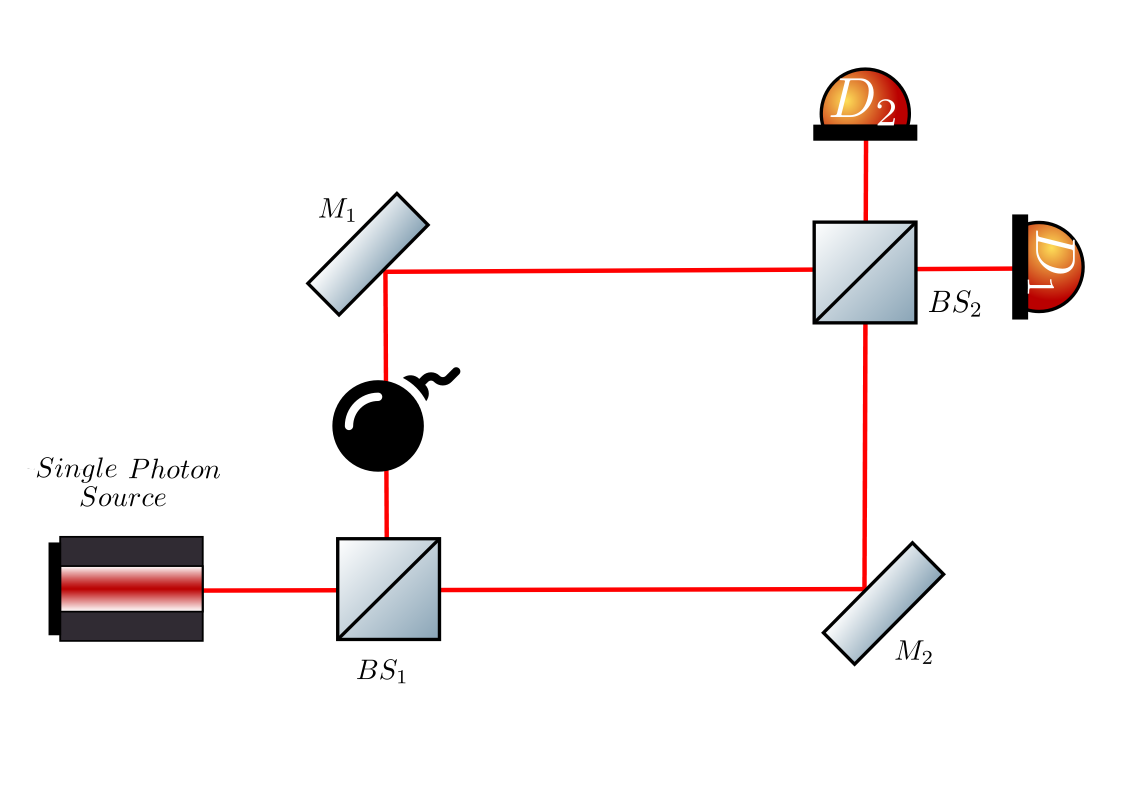
\includegraphics[width=\linewidth]{machzenhderbomb.jpg}
\caption{Elitzur-Vaidman's bomb detector}
\label{fig:BS2}
\end{figure}

to analyze this case we will simply repeat the calculations we did above this time having a perfect absorber in the also vertical arm of the interferometer as the figure shows , we also need to consider that once the photon is absorbed the optical elements do not interact with it , we will denote an absorbed photon using the $\ket{Abs}$ state
  
$\ket{1}\xrightarrow{\text{BS1}}\cos(\theta_{1})\ket{1}+i\sin(\theta_{1})\ket{2}\xrightarrow{\text{Bomb}}\cos(\theta_{1})\ket{1}+i\sin(\theta_{1})\ket{Abs}\xrightarrow{\text{Mirrors}}i\cos(\theta_{1})\ket{2}+i\sin(\theta_{1})\ket{Abs}\xrightarrow{\text{BS2}}i\cos(\theta_{1})\cos(\theta_{2})\ket{2}-\cos(\theta_{1})\sin(\theta_{2})\ket{1}+i\sin(\theta_{1})\ket{Abs}$.

so the probabilities to be absorbed or detected at either $D_{1}$ or $D_{2}$ are given by:

$P_{D1}=\cos^2(\theta_{1}) \sin^2(\theta_{2}) $.

$P_{D2}=\cos^2(\theta_{1}) \cos^2(\theta_{2})$.

$P_{Abs}=\sin^2(\theta_{1})$.

Let's again consider the case where $\theta_{1}=\theta_{2}=\frac{\pi}{4}$ then:

$P_{D1}=\frac{1}{4} $.

$P_{D2}=\frac{1}{4}$.

$P_{Abs}=\frac{1}{2}$.

So having a detection in $D_{2}$ would indicate that there's an object in one of the arms of the interferometer , this is often called non-interactive measurements because we can infer information of the object from the photons that did not interact with it , a pertinent comment may be that while this is true we still need many events to actually obtain information from this setups , and at least in this case about 1/4 of the events will interact with the object even though we do not get information from them

\vspace
{0.3cm}


\section{The Single Photon Mach-Zehnder with an  \\ imperfect absorber}

This section and the next ones are based on the treatment done by Zurika B. and Rosas-Ortiz \cite{tesis zuri} and the work done by Azuma \cite{Azuma}.Let's consider an object such that $\alpha'$ and $\beta'$ are its absorption and transmission coefficients, thus:
\vspace
{0.2cm}

$|\alpha'|^2 + |\beta'|^2 = 1$  


And we can write said coefficients in polar form as:

$\alpha'=\alpha e^{i \theta}$ 

$\beta'=\beta e^{i \gamma}$
\vspace
{0.2cm}



We will use the same Horizontal-Vertical basis and our source will start in the state $\ket{1}$ and we will have our imperfect absorber in the vertical path 

Our imperfect absorber can either transmit with probability $|\beta'|^2$ or absorb with probability $|\alpha'|^2$ ,such that when encountered with this object our states become:



$\ket{2}\xrightarrow[\text{Absorber}]{\text{Imperfect}}\alpha' \ket{abs} +\beta' \ket{2} $

$\ket{1}\xrightarrow[\text{Absorber}]{\text{Imperfect}}\alpha' \ket{abs} +\beta' \ket{1} $

\vspace
{0.3cm}
with this information we can now go on with our calculations:
\vspace
{0.3cm}

$\ket{1}\xrightarrow{\text{BS1}}\cos(\theta_{1})\ket{1}+i\sin(\theta_{1})\ket{2}\xrightarrow[\text{Absorber}]{\text{Imperfect }}\cos(\theta_{1})\ket{1}+i\sin(\theta_{1})(\alpha' \ket{abs} +\beta' \ket{2} )
\xrightarrow{\text{Mirrors}}i\cos(\theta_{1})\ket{2}+i \sin(\theta_{1})\alpha'\ket{abs}-\sin(\theta_{1})\beta'\ket{1}\xrightarrow{\text{BS2}}-
(\cos(\theta_{1})\sin(\theta_{2})+\beta' \sin(\theta_{1})\cos(\theta_{2}))\ket{1}+i \alpha' \sin(\theta_{1})\ket{abs}+i(\cos(\theta_{1})\cos(\theta_{2})-\sin(\theta_{1})\sin(\theta_{2})\beta')\ket{2}$.

\vspace
{0.3cm}

Therefore the probabilities are given by:

$P_{2D1}=|\cos(\theta_{1})\sin(\theta_{2})+\beta' \sin(\theta_{1})\cos(\theta_{2})|^2$.

$P_{2D2}=|\cos(\theta_{1})\cos(\theta_{2})-\beta' \sin(\theta_{1})\sin(\theta_{2})|^2$.

$P_{2Abs}=|\alpha' \sin(\theta_{1})|^2$.

\vspace
{0.3cm}

If we consider the exact same procedure but this time we put our imperfect absorber on the other arm of the interferometer we obtain:
\vspace
{0.3cm}

$P_{1D1}=|\cos(\theta_{1})\sin(\theta_{2})\beta' +\sin(\theta_{1})\cos(\theta_{2})|^2$.

$P_{1D2}=|\sin(\theta_{1})\sin(\theta_{2})-\beta' \cos(\theta_{1})\cos(\theta_{2})|^2$.

$P_{1Abs}=|\alpha' \cos(\theta_{1})|^2$.

\vspace
{0.3cm}

Observing the probabilities are different we can obtain the difference between them:

\vspace
{0.3cm}

$P_{1D1}-P_{1D2}=(1-\beta^2)\left(\frac{\cos(2 \theta_{1})-\cos(2 \theta_{2})}{2}\right)$.

$P_{2D1}-P_{2D2}=(1-\beta^2)\left(\frac{\cos(2 \theta_{1})+\cos(2 \theta_{2})}{2}\right)$.

\vspace
{0.3cm}

From there we can say that the probabilities are the same only when :

a)$\beta=1  $ which means a totally transparent object.

b)$\cos(2 \theta_{2})+\cos(2\theta_{1})=\cos(2 \theta_{1})-\cos(2\theta_{2})=0$   which means   $\theta_{1}=\theta_{2}=\frac{\pi}{4}\pm 2n\pi$
.

\vspace
{0.3cm}
We can also obtain an expression for one of the angles in terms of the probabilities

\vspace
{0.3cm}
$\theta_{2}=\frac{1}{2}(\acos((P_{1D2}-P_{1D1})-(P_{1D1}-P_{2D1})))$.

$\theta_{1}=\frac{1}{2}(\acos((P_{1D2}-P_{1D1})+(P_{1D1}-P_{2D1})))$.
\vspace
{0.3cm}

\section{Mach-Zenhder with BS as imperfect absorber}

We will now study the case of a BS as an imperfect absorber , we will also consider imperfect mirrors such that $\gamma \neq \frac{\pi}{2}$, just like in the previous cases we will first consider our imperfect absorber in the vertical path

\begin{figure}[h!]
\centering
\includegraphics[width=\linewidth,height=6.5 cm]{machzenhderbs.jpg}
\caption{Mach Zehnder with a BS as imperfect absorber}
\label{fig:BS2}
\end{figure}

\vspace{10 cm}

Our BS transmission coefficient is $\cos(\theta_{o})$ and its reflection coefficient is $i\sin(\theta_{o})$ when a state interacts with our imperfect absorber 

$\ket{2}\xrightarrow[\text{Absorber}]{\text{Imperfect}}i\sin(\theta_{o}) \ket{abs} +\cos(\theta_{o}) \ket{2} $

$\ket{1}\xrightarrow[\text{Absorber}]{\text{Imperfect}}i\sin(\theta_{o}) \ket{abs} +\cos(\theta_{o}) \ket{1} $

We consider the reflected photon to be lost since it goes out of our interferometer , and we denote that "lost photon" state by $\ket{abs}$, we that in mind now we can begin our calculation which is analogous to the ones from the previous sections


$\ket{1}\xrightarrow{\text{BS1}}\cos(\theta_{1})\ket{1}+i\sin(\theta_{1})\ket{2}\xrightarrow{\text{BS}}\cos(\theta_{1})\ket{1}+i\sin(\theta_{1})(\cos(\theta_{o})\ket{2}+i\sin(\theta_{o})\ket{abs}\xrightarrow{\text{Mirrors}}\cos(\theta_{1})e^{i\gamma_{1}}\ket{2}+i\sin(\theta_{1})\cos(\theta_{o})e^{i\gamma_{2}}\ket{1}-\sin(\theta_{1})\sin(\theta_{o})\ket{abs}\xrightarrow{\text{BS2}}\cos(\theta_{1})e^{i\gamma_{1}}(\cos(\theta_{2})\ket{2}+i\sin(\theta_{2})\ket{1})+i\sin(\theta_{1})\cos(\theta_{o})e^{i\gamma_{2}}(\cos(\theta_{2})\ket{1}+i\sin(\theta_{2})\ket{2})-\sin(\theta_{1})\sin(\theta_{o})\ket{abs}\xrightarrow{\text{grouping}}(\cos(\theta_{1})e^{i\gamma_{1}}\cos(\theta_{2})-\sin(\theta_{1})\sin(\theta_{2})\cos(\theta_{o})e^{i\gamma_{2}})\ket{2}-\sin(\theta_{1})\sin(\theta_{o})\ket{abs}+(i\cos(\theta_{1})\sin(\theta_{2})e^{i\gamma_{1}}+i \sin(\theta_{1})\cos(\theta_{o})\cos(\theta_{2})e^{i\gamma_{2}})\ket{1}$

\vspace{0.3cm}

so probabilities are given by:


\begin{figure}[h!]
\centering
\begin{subfigure}[b]{0.45\linewidth}
\includegraphics[width=\linewidth,height=2.8 cm]{P1abs.png}
\caption{$P_{2Abs}$}
\label{fig:BS2}
\end{subfigure}
\begin{subfigure}[b]{0.45\linewidth}
\includegraphics[width=\linewidth,height=2.8 cm]{P1d1.png}
\caption{$P_{2D1}$}
\label{fig:westminster_aerea}
\end{subfigure}
\begin{subfigure}[b]{0.45\linewidth}
\includegraphics[width=\linewidth,height=2.8 cm]{P1d2.png}
\caption{$P_{2D1}$}
\label{fig:BS2}
\end{subfigure}
\caption{Probability distributions with imperfect absorber in vertical path and $\theta_{o}=\frac{\pi}{3}$ y $\gamma_{2}-\gamma_{1}=\pi$}
\label{fig:westminster}
\end{figure} 

\vspace{9 cm}

$P_{2D1}=|ie^{i\gamma_{1}}\cos(\theta_{1})\sin(\theta_{2})+i e^{i\gamma_{2}}\cos(\theta_{o}) \sin(\theta_{1})\cos(\theta_{2})|^2$.

\vspace{0.1cm}

$P_{2D2}=|\cos(\theta_{1})\cos(\theta_{2})e^{i\gamma_{1}}- e^{i\gamma_{2}}\cos(\theta_{o}) \sin(\theta_{1})\sin(\theta_{2})|^2$.

\vspace{0.1cm}

$P_{2Abs}=|\sin(\theta_{o}) \sin(\theta_{1})|^2$.

\vspace{0.3cm}

Repeating the exact same calculation with the object in the horizontal path we obtain the following probabilities:


\begin{figure}[h!]
\centering
\begin{subfigure}[b]{0.45\linewidth}
\includegraphics[width=\linewidth]{P11abs.png}
\caption{$P_{1Abs}$}
\label{fig:BS1}
\end{subfigure}
\begin{subfigure}[b]{0.45\linewidth}
\includegraphics[width=\linewidth]{P11d1.png}
\caption{$P_{1D1}$}
\label{fig:westminster_aerea}
\end{subfigure}
\begin{subfigure}[b]{0.45\linewidth}
\includegraphics[width=\linewidth]{P11d2.png}
\caption{$P_{1D1}$}
\label{fig:BS1}
\end{subfigure}
\caption{Probabilities distribution in the Horizontal path for $\theta_{o}=\frac{\pi}{3}$ y $\gamma_{2}-\gamma_{1}=\pi$}
\label{fig:westminster}
\end{figure} 

\vspace{5cm}

$P_{1D1}=|ie^{i\gamma_{1}}\cos(\theta_{1})\sin(\theta_{2})\cos(\theta_{o})+i e^{i\gamma_{2}}\sin(\theta_{1})\cos(\theta_{2})|^2$.

\vspace{0.1cm}

$P_{1D2}=|\cos(\theta_{1})\cos(\theta_{o})\cos(\theta_{2})e^{i\gamma_{1}}-e^{i\gamma_{2}} \sin(\theta_{1})\sin(\theta_{2})|^2$.

\vspace{0.1cm}

$P_{1Abs}=|\sin(\theta_{o}) \cos(\theta_{1})|^2$.

\vspace{0.3cm}

This analysis is totally consistent with Zurika's \cite{tesis de Zurika} when one takes the case $\beta'=\cos(\theta_{o})$ and $\alpha'=\sin(\theta_{o})$ however this case has a little advantage and that is that our "absorbed" photon , is not absorbed but goes out of our interferometer so we can actually measure all outputs of the interferometer by placing a detector say $D_{abs}$ in the path the "lost photon" would follow
 
\section{Optical Chopper as perfect absorber }
 
 \begin{figure}[h!]
\centering
\includegraphics[width=\linewidth]{machzenhderchopper.jpg}
\caption{Mach-Zehnder with an optical chopper as an imperfect absorber}
\label{fig:BS2}
\end{figure}
  An optical chopper is a device that periodically interrupts light, it is usually a disk with holes rotating with a certain frequency (which can vary in time) , from it's definition we can infer that it can be modeled using a square wave which can be written as  $f(t)=\frac{sgn(\sin(wt))+1}{2}$,where $\omega$ is the angular frequency of the optical chopper multiplied by the number of "hole-material" pairs which for now we assume are the same size, we will be ignoring diffraction effects , also from the way we're deciding to model the chopper and the fact that products of square waves are square waves we can see that the effect of an optical chopper would be the same as that of many 

We can model our optical chopper by using a diagonal matrix in our base:

$C
=\begin
{pmatrix} \frac{sgn
(\sin(wt
))+1}{2} & 0 \\ 0 & \frac{sgn
(\sin(wt
))+1}{2} \end
{pmatrix}$.

Ideally we want this matrix to be unitary , which will be checked right away:

$|f|^2=\frac{(sgn(\sin(wt)+1)^2}{4}$.

the sign function squared is always one so

$|f|^2=\frac{2(1+sgn
(\sin(wt
)))}{4}$.

$|f|^2=f$.


from there we can see that it is a unitary matrix whenever the sine is in the positive cycle, and it becomes null in the negative cycle , that happens because in the negative cycle we have total absorption, the absorption coefficient would  be: 


$a=1-f$.

$a=\frac{1-sgn(\sin(wt))}{2}$.


$|a|^2=\frac{2(1-sgn(\sin(wt)))}{4}$.

$|a|^2=a$.

We will now analyze a Mach-Zehnder interferometer using a chopper as an imperfect absorber, the chopper will be placed on the vertical path , and our photon will go into the interferometer using the horizontal path



$\ket{1}\xrightarrow{\text{BS1}}\cos(\theta_{1})\ket{1}+i\sin(\theta_{1})\ket{2}\xrightarrow{\text{Chopper}}\cos(\theta_{1})\ket{1}+i\sin(\theta_{1})f\ket{2}+i\sin(\theta_{1})a\ket{abs}\xrightarrow{\text{Mirrors}}\cos(\theta_{1})e^{i\gamma_{1}}\ket{2}+i\sin(\theta_{1})f e^{i\gamma_{2}}\ket{1}+i\sin(\theta_{1})a\ket{abs}\xrightarrow{\text{BS2}}\cos(\theta_{1})e^{i\gamma_{1}}(\cos(\theta_{2})\ket{2}+i\sin(\theta_{2})\ket{1})+i\sin(\theta_{1})e^{i\gamma_{2}}f(\cos(\theta_{2})\ket{1}+i\sin(\theta_{2})\ket{2})+i\sin(\theta_{1})a\ket{abs}\xrightarrow{\text{Grouping}}i(e^{i\gamma_{1}}\cos(\theta_{1})\sin(\theta_{2})+f e^{i\gamma_{2}}\sin(\theta_{1})\cos(\theta_{2}))\ket{1}+(\cos(\theta_{1})\cos(\theta_{2}) e^{i\gamma_{1}}-\sin(\theta_{1})\sin(\theta_{2})f e^{i \gamma_{2}})\ket{2}+i\sin(\theta_{1})a\ket{abs}$.



From there we can see the detection probabilities are given by : 

\begin{figure}[h!]
\centering

\begin{subfigure}[b]{0.45\linewidth}
\includegraphics[width=\linewidth,height=3.5cm]{Pc2Abs.png}
\caption{$P_{1Abs}$}
\label{fig:BS1}
\end{subfigure}
\begin{subfigure}[b]{0.45\linewidth}
\includegraphics[width=\linewidth,,height=3.5cm]{Pc2D21.png}
\caption{$P_{2D1}$ in the first cycle }
\label{fig:BS1}
\end{subfigure}
\begin{subfigure}[b]{0.45\linewidth}
\includegraphics[width=\linewidth,height=3.5cm]{Pc2D22.png}
\caption{$P_{2D1}$ in the second cycle}
\label{fig:BS1}
\end{subfigure}
\begin{subfigure}[b]{0.45\linewidth}
\includegraphics[width=\linewidth,height=3.5cm]{Pc2D11.png}
\caption{$P_{2D1} $ in the first cycle}
\label{fig:westminster_aerea}
\end{subfigure}
\begin{subfigure}[b]{0.45\linewidth}
\includegraphics[width=\linewidth,height=3.5cm]{Pc2D12.png}
\caption{$P_{2D1} $ in the second cycle }
\label{fig:BS1}
\end{subfigure}
\caption{Probability Distribution for $\gamma_{2}-\gamma_{1}=\frac{\pi}{2}$ in the vertical path}
\label{fig:westminster}
\end{figure}

\vspace
{15 cm}

 $P_{2D1}=|e^{i\gamma_{1}}\cos(\theta_{1})\sin(\theta_{2})+f e^{i\gamma_{2}}\sin(\theta_{1})\cos(\theta_{2})|^2$.
 
$P_{2D2}=|\cos(\theta_{1})\cos(\theta_{2})e^{i\gamma_{1}}- f \sin(\theta_{1})\sin(\theta_{2})e^{i\gamma_{2}}|^2$.

$P_{2Abs}=|a \sin(\theta_{1})|^2$.

Which can be written as:

$P_{2D1}=\cos^2(\theta_{1})\sin^2(\theta_{2})+f^2 \sin^2(\theta_{1})\cos^2(\theta_{2})+\frac{f \sin(2\theta_{1})\sin(2\theta_{2})\cos(\gamma_{1}-\gamma_{2})}{2}$.

$P_{2D2}=\cos^2(\theta_{1})\cos^2(\theta_{2})+ f^2 \sin^2(\theta_{1})\sin^2(\theta_{2})-\frac{f \sin(2\theta_{1})\sin(2\theta_{2})\cos(\gamma_{1}-\gamma_{2})}{2}$.

$P_{2Abs}=a^2 \sin^2(\theta_{1})$.


By the exact same procedure having the chopper in the horizontal path , one can obtain the following results
 
\begin{figure}[h!]
\centering
\begin{subfigure}[b]{0.35\linewidth}
\includegraphics[width=\linewidth,height=3 cm]{Pc1Abs.png}
\caption{$P_{1Abs}$}
\label{fig:BS1}
\end{subfigure}
\begin{subfigure}[b]{0.35\linewidth}
\includegraphics[width=\linewidth,height=3 cm]{Pc1D21.png}
\caption{$P_{1D1}$ in the first cycle }
\label{fig:BS1}
\end{subfigure}
\begin{subfigure}[b]{0.35\linewidth}
\includegraphics[width=\linewidth,height=3 cm]{Pc1D22.png}
\caption{$P_{1D1}$ in the second cycle}
\label{fig:BS1}
\end{subfigure}
\begin{subfigure}[b]{0.35\linewidth}
\includegraphics[width=\linewidth,height=3 cm]{Pc1D11.png}
\caption{$P_{1D1} $ in the first cycle}
\label{fig:westminster_aerea}
\end{subfigure}
\begin{subfigure}[b]{0.35\linewidth}
\includegraphics[width=\linewidth,height=3 cm]{Pc1D12.png}
\caption{$P_{1D1} $in the second cycle }
\label{fig:BS1}
\end{subfigure}
\caption{Probability distribution for the horizontal path and  $\gamma_{2}-\gamma_{1}=\frac{\pi}{2}$}
\label{fig:westminster}
\end{figure}

\vspace{15cm}

$P_{1D1}=\cos^2(\theta_{1})\sin^2(\theta_{2})f^2+ \sin^2(\theta_{1})\cos^2(\theta_{2})+\frac{f \sin(2\theta_{1})\sin(2\theta_{2})\cos(\gamma_{1}-\gamma_{2})}{2}$.

$P_{1D2}=\cos^2(\theta_{1})\cos^2(\theta_{2})f^2+ \sin^2(\theta_{1})\sin^2(\theta_{2})-\frac{f \sin(2\theta_{1})\sin(2\theta_{2})\cos(\gamma_{1}-\gamma_{2})}{2}$.

$P_{2Abs}=a^2 \cos^2(\theta_{1})$.\\


we already showed that $f^2=f$ using this and subtracting:

$P_{1D1}-P_{1D2}=(1-f)\left(\frac{\cos(2 \theta_{1})-\cos(2 \theta_{2})}{2}\right)$.

$P_{2D1}-P_{2D2}=(1-f)\left(\frac{\cos(2 \theta_{1})+\cos(2 \theta_{2})}{2}\right)$.

Since $1-f=a$

$P_{1D1}-P_{1D2}=(a)\left(\frac{\cos(2 \theta_{1})-\cos(2 \theta_{2})}{2}\right)$.

$P_{2D1}-P_{2D2}=(a)\left(\frac{\cos(2 \theta_{1})+\cos(2 \theta_{2})}{2}\right)$.

 From there we can obtain either $\theta_{1}$  or $\theta_{2}$ :

$P_{1D1}-P_{1D2}+P_{2D1}-P_{2D2}=(a)(\cos(2 \theta_{1}))$.

$P_{1D1}-P_{1D2}-P_{2D1}-P_{2D2}=(-a)(\cos(2 \theta_{2}))$.


$ \theta_{1}=\frac{1}{2}\acos(\frac{P_{1D1}-P_{1D2}+P_{2D1}-P_{2D2}}{a})$ .

$\theta_{2}=\frac{1}{2}\acos(\frac{P_{1D1}-P_{1D2}-P_{2D1}-P_{2D2}}{a})$.

\section{Optical Chopper as imperfect absorber}

Previously we considered the "material" part of the chopper as a perfect absorber, we will now generalize that to when it is an imperfect absorber, this can be done quite simply by defining :
 
 \vspace{1 cm}
 
 $f_{hole}=\frac{1+sgn(\sin(wt))}{2}$.

$f_{material}=\left(\frac{1-sgn(\sin(wt))}{2} \right)\beta$.

$f=f_{material}+f_{hole}$.



\vspace{1cm}

where $\beta$ is the transmission coefficient of the material part of our chopper, which could be a function of  $\omega$ or t in this analysis,the matrix used to describe our chopper is the same as in the previous section:

 
\vspace{1cm}

$C=\begin{pmatrix} f & 0 \\ 0 & f \end{pmatrix}$.

\vspace{1 cm}

we define:

\vspace{0.5cm}

$a=\left(\frac{1-sgn(\sin(wt))}{2}\right) \alpha$.
\vspace{0.5cm}

where $\alpha$ is the absorption coefficient of the material part of our chopper , by using this notation we have the exact same case as in the previous section , except this time $f^2 \neq 1$ :

$|a|^2=a$ $\alpha$.

$|f_{material}|^2=f_{material}$ $\beta$.

Which we can generalize to obtain:

$|a|^n=a$ $\alpha^{n-1}$.

$|f_{material}|^n=f_{material}$ $\beta^{n-1}$.

so we have:

$|f|^2=  \frac{\abs{\alpha}^2}{2} sgn(\sin(wt)) +\frac{1+\abs{\beta}^2}{2}$ .

\vspace{0.5cm}

Substituting in the previous section yields:
\begin{figure}[h!]
\centering
\begin{subfigure}[b]{0.40\linewidth}
\includegraphics[width=\linewidth,height=3.5 cm]{p1cabs.png}
\caption{$P_{1Abs}$}
\label{fig:BS1}
\end{subfigure}
\begin{subfigure}[b]{0.40\linewidth}
\includegraphics[width=\linewidth,height=3.5 cm]{p1cd21.png}
\caption{$P_{1D1}$ in the first cycle }
\label{fig:BS1}
\end{subfigure}
\begin{subfigure}[b]{0.40\linewidth}
\includegraphics[width=\linewidth,height=3.5 cm]{p1cd22.png}
\caption{$P_{1D1}$ in the second cycle}
\label{fig:BS1}
\end{subfigure}
\begin{subfigure}[b]{0.40\linewidth}
\includegraphics[width=\linewidth,height=3.5 cm]{p1cd11.png}
\caption{$P_{1D1} $ in the first cycle}
\label{fig:westminster_aerea}
\end{subfigure}
\begin{subfigure}[b]{0.40\linewidth}
\includegraphics[width=\linewidth,height=3.5 cm]{p1cd12.png}
\caption{$P_{1D1} $ in the second cycle }
\label{fig:BS1}
\end{subfigure}
\caption{Probability Distribution in the horizontal path with  $\gamma_{2}-\gamma_{1}=0 $ y $\beta=0.5$}
\label{fig:westminster}
\end{figure}

\vspace{12cm}

$P_{1D1}=\cos^2(\theta_{1})\sin^2(\theta_{2})\abs{f}^2+ \sin^2(\theta_{1})\cos^2(\theta_{2})+\frac{\Re{f} \sin(2\theta_{1})\sin(2\theta_{2})\cos(\gamma_{1}-\gamma_{2})}{2}$.

$P_{1D2}=\cos^2(\theta_{1})\cos^2(\theta_{2})\abs{f}^2+ \sin^2(\theta_{1})\sin^2(\theta_{2})-\frac{\Re{f} \sin(2\theta_{1})\sin(2\theta_{2})\cos(\gamma_{1}-\gamma_{2})}{2}$.

$P_{1Abs}=\abs{\alpha}^2 \cos^2(\theta_{1})$.\\



When the optical chopper is in the vertical path we obtain:

\begin{figure}[h!]
\centering
\begin{subfigure}[b]{0.40\linewidth}
\includegraphics[width=\linewidth,height=3.5 cm]{pcabs.png}
\caption{$P_{1Abs}$}
\label{fig:BS1}
\end{subfigure}
\begin{subfigure}[b]{0.40\linewidth}
\includegraphics[width=\linewidth,height=3.5 cm]{pcd21.png}
\caption{$P_{2D1}$ in the first cycle }
\label{fig:BS1}
\end{subfigure}
\begin{subfigure}[b]{0.40\linewidth}
\includegraphics[width=\linewidth,height=3.5 cm]{pcd22.png}
\caption{$P_{2D1}$ in the second cycle}
\label{fig:BS1}
\end{subfigure}
\begin{subfigure}[b]{0.40\linewidth}
\includegraphics[width=\linewidth,height=3.5 cm]{pcd11.png}
\caption{$P_{2D1} $ in the first cycle}
\label{fig:westminster_aerea}
\end{subfigure}
\begin{subfigure}[b]{0.40\linewidth}
\includegraphics[width=\linewidth,height=3.5 cm]{pcd12.png}
\caption{$P_{2D1} $ in the second cycle }
\label{fig:BS1}
\end{subfigure}
\caption{Probability Distribution for the vertical path with  $\gamma_{2}-\gamma_{1}=0 $ y $\beta=0.5$}
\label{fig:westminster}
\end{figure}
\vspace{5cm}
$P_{2D1}=\cos^2(\theta_{1})\sin^2(\theta_{2})+\abs{f}^2 \sin^2(\theta_{1})\cos^2(\theta_{2})+\frac{\Re{f} \sin(2\theta_{1})\sin(2\theta_{2})\cos(\gamma_{1}-\gamma_{2})}{2}$.

$P_{2D2}=\cos^2(\theta_{1})\cos^2(\theta_{2})+ \abs{f}^2 \sin^2(\theta_{1})\sin^2(\theta_{2})-\frac{\Re{f} \sin(2\theta_{1})\sin(2\theta_{2})\cos(\gamma_{1}-\gamma_{2})}{2}$.

$P_{2Abs}=\abs{\alpha}^2 \sin^2(\theta_{1})$.


\section{n Beam Splitters as imperfect absorber }
\vspace{1 cm}
\begin{figure}[h!]
\centering
\includegraphics[width=\linewidth]{machzenhderBSS.jpg}
\caption{Mach Zehnder with N BS as imperfect absorber}
\label{fig:BS2}
\end{figure}

We begin analyzing what happens if our initial state goes through several BS assuming the reflected photon is "lost" :


$B_{1}\ket{1}=\cos(\theta_{1})\ket{1}+i\sin(\theta_{1})\ket{abs}$.

$B_{1}\ket{2}=\cos(\theta_{1})\ket{2}+i\sin(\theta_{1})\ket{abs}$.

The next BS only act on the transmitted photon so:

$B_{2}(\cos(\theta_{1})\ket{1}+i\sin(\theta_{1})\ket{abs})=\cos(\theta_{1})B_{2}\ket{1}+i\sin(\theta_{1})\ket{abs}$.

$B_{2}(\cos(\theta_{1})\ket{2}+i\sin(\theta_{1})\ket{abs})=\cos(\theta_{1})B_{2}\ket{2}+i\sin(\theta_{1})\ket{abs}$.

$B_{2}B_{1}\ket{2}=\cos(\theta_{1})\cos(\theta_{2})\ket{2}+i A'\ket{abs}$

$B_{2}B_{1}\ket{1}=\cos(\theta_{1})\cos(\theta_{2})\ket{1}+i A\ket{abs}$

Then the next BS does the same


$B_{3}B_{2}B_{1}\ket{1}=\cos(\theta_{1})\cos(\theta_{2})\cos(\theta_{3})\ket{1}+iB\ket{abs}$

$B_{3}B_{2}B_{1}\ket{2}=\cos(\theta_{1})\cos(\theta_{2})\cos(\theta_{3})\ket{2}+iB'\ket{abs}$

so after n BS :

$B^{n}=B_{n}...B_{3}B_{2}B_{1}\ket{1}=\cos(\theta_{1})\cos(\theta_{2})\cos(\theta_{3})....\cos(\theta_{n})\ket{1}+i C\ket{abs}$

$B^{n}=B_{n}...B_{3}B_{2}B_{1}\ket{2}=\cos(\theta_{1})\cos(\theta_{2})\cos(\theta_{3})....\cos(\theta_{n})\ket{2}+i C'\ket{abs}$

We can obtain C and C' by asking the probabilities to add to unity:

$B^{n}\ket{1}=\prod_{i=1}^{n} \cos(\theta_{i})\ket{1}+i D\ket{abs}  $


$B^{n}\ket{2}=\prod_{i=1}^{n} \cos(\theta_{i})\ket{2}+i D'\ket{abs}  $



$D'=D=\sqrt{1-\prod_{i=1}^{n}\cos^2(\theta_{i})}$


We now use this as a imperfect absorber in the vertical path:

$\ket{1}\xrightarrow{\text{BS1}}\cos(\theta_{1})\ket{1}+i\sin(\theta_{1})\ket{2}\xrightarrow{{B^{n}}}\cos(\theta_{1})\ket{1}+i\sin(\theta_{1})\prod_{i=3}^{n} \cos(\theta_{i})\ket{2}-\sin(\theta_{1})\sqrt{1-\prod_{i=3}^{n}\cos^2(\theta_{i})}\ket{Abs} \xrightarrow{{Mirrors}}\cos(\theta_{1})  e^{i \gamma_{1}}\ket{2}+i\sin(\theta_{1})\prod_{i=3}^{n} \cos(\theta_{i}) e^{i \gamma_{2}}\ket{1}-\sin(\theta_{1})\sqrt{1-\prod_{i=3}^{n}\cos^2(\theta_{i})}\ket{Abs} \xrightarrow{{BS2}} (\cos(\theta_{1})\cos(\theta_{2})e^{i \gamma_{1}}-\sin(\theta_{1})\sin(\theta_{2})e^{i \gamma_{2}}\prod_{i=3}^{n} \cos(\theta_{i}))\ket{2}+i(\cos(\theta_{1})\sin(\theta_{2})e^{i \gamma_{1}}+\cos(\theta_{2})\sin(\theta_{1})e^{i \gamma_{2}}\prod_{i=3}^{n} \cos(\theta_{i}))\ket{1}-\sin(\theta_{1})\sqrt{1-\prod_{i=3}^{n}\cos^2(\theta_{i})}\ket{Abs} $.

the probabilities of detection are given by:

$P_{D1}=|\cos(\theta_{1})\sin(\theta_{2})e^{i \gamma_{1}}+\cos(\theta_{2})\sin(\theta_{1})e^{i \gamma_{2}}\prod_{i=3}^{n} \cos(\theta_{i})|^2$.

$P_{D2}=|\cos(\theta_{1})\cos(\theta_{2})e^{i \gamma_{1}}-\sin(\theta_{1})\sin(\theta_{2})e^{i \gamma_{2}}\prod_{i=3}^{n} \cos(\theta_{i})|^2$.

$P_{Abs}=\sin^2(\theta_{1})(1-\prod_{i=3}^{n}\cos^2(\theta_{i}))$.

\section{Analysis with phase retarders }

The interferometer is an instrument quite hard to align , in most cases alignment is a little of , we can characterize just how off this alignment is by considering the effects of phase retarders on the interferometer and having those predictions compared with the actual interferometer (without phase retarders), a wave retarder's  matrix representation is:



 $Retarder=\begin
{pmatrix} e^
{i c} & 0\\0& e^
{i k }\end
{pmatrix}$.

Let's see the effect of such an optical device in our setup:

$\ket{1}\xrightarrow{\text{BS1}}\cos(\theta_{1})\ket{1}+i\sin(\theta_{1})\ket{2}\xrightarrow[\text{Absorber}]{\text{Imperfect }}cos(\theta_{1})\ket{1}+i\sin(\theta_{1})(\alpha' \ket{abs} +\beta' \ket{2} )\xrightarrow[\text{Retarder}]{\text{Phase}}\cos(\theta_{1})e^{ic}\ket{1}+i\beta'\sin(\theta_{1}) e^{ik}\ket{2} +i\alpha'\sin(\theta_{1}) \ket{abs}\xrightarrow{\text{Mirrors}} \cos(\theta_{1})e^{i(\gamma_{1}'+c)}\ket{2}+i \sin(\theta_{1})\alpha'\ket{abs}+i\sin(\theta_{1})\beta'e^{i(\gamma_{2}'+k)}\ket{1}$.

We can stop here by noticing that making $\gamma_{2}'+k=\gamma_{2}$ and $\gamma_{1}'+c=\gamma_{1}$ we have the exact same case as in our previous sections , like in the section of a BS as an imperfect absorber with  $\beta'=cos(\theta_{o})$ and $\alpha'=i\sin(\theta_{o})$ so our model that makes use of the general matrix of a mirror instead of using the more popular perfect mirror matrix $M=\begin{pmatrix} i & 0\\0& i\end{pmatrix}$ has the  effect of a phase retarder included , allowing us to study misalignment.

 \section{Analysis of N Intereferometers }
 
 the notation previously used is not popular when dealing with nested interferometers , in order to be consistent with the existing literature we will use the same notation as Kwait et al.\cite{5}, where we have an interferometer  like the one in the following figure:
 
\begin{figure}[h!]
\centering
\includegraphics[width=\linewidth]{baseAzuma.png}
\caption{Nested Mach-Zehnders  with imperfect absorbers}
\label{fig:BS2}
\end{figure}
 
 We will still use a binary basis , but instead of using the Horizontal-Vertical, it will be a path A- path B basis, that is a "up-down" basis, we will use $\ket{2}$ for path b and $\ket{1}$ for path a, one of the main advantages of this basis is that the mirror matrices are diagonal in this basis , beacuse they keep our photon on the same path, We will model our imperfect absorber using a non-unitary diagonal matrix just as was done by  Azuma \cite{9}  
 
 Azuma used a matrix of the form:
 
  $A_{Azuma}=\begin{pmatrix} \sqrt{n} & 0\\0& 1\end{pmatrix}$.

Since we are using a BS as an imperfect absorber a more suitable option would be :

 $A_{BS}=\begin{pmatrix} \cos(n) & 0\\0& 1\end{pmatrix}$.


The final state can be obtained by applying all of the operators to the initial state which will be $\ket{2}$, Let's first consider that we have no imperfect absorbers on the interferometer, then the only operators acting on the state are $BS$ then:

$BS_{i} \times BS_{i+1}=\begin{pmatrix} \cos(\theta_{i}) & i \sin(\theta_{i}) \\ i \sin(\theta_{i}) & \cos(\theta_{i}) \end{pmatrix}  
\begin{pmatrix} \cos(\theta_{i+1}) & i \sin(\theta_{i+1}) \\ i \sin(\theta_{i+1}) & \cos(\theta_{i+1}) \end{pmatrix}$

$BS_{i} \times BS_{i+1}=\begin{pmatrix} \cos(\theta_{i})\cos(\theta_{i+1})-\sin(\theta_{i})\sin(\theta_{i+1}) & i (\cos(\theta_{i+1})\sin(\theta_{i})+\cos(\theta_{i})\sin(\theta_{i+1})) \\ i (\cos(\theta_{i+1})\sin(\theta_{i})+\cos(\theta_{i})\sin(\theta_{i+1}))& \cos(\theta_{i})\cos(\theta_{i+1})-\sin(\theta_{i})\sin(\theta_{i+1}) \end{pmatrix}$

Which can be rewritten as:

$BS_{i} \times BS_{i+1}=\begin{pmatrix} \cos(\theta_{i}+\theta_{i+1}) & i \sin(\theta_{i}+\theta_{i+1}) \\ i \sin(\theta_{i}+\theta_{i+1}) & \cos(\theta_{i}+\theta_{i+1}) \end{pmatrix} $

If we assume N BS that are identical:

$BS^{N}=\begin{pmatrix} \cos(N\theta) & i \sin(N\theta) \\ i \sin(N\theta) & \cos(N\theta) \end{pmatrix}$

Let's assume $\theta=\frac{\pi}{2N}$ so we have:

$BS^{N}=\begin{pmatrix} 0 & i  \\ i  & 0 \end{pmatrix}$

So we will always detect the photon in the path that's not the the one we sent our photon in ,with this in mind let's see what happens with this particular $\theta$ when we do have imperfect absorbers. the state first goes through a BS, then one of the imperfect absorbers and then another BS, it keeps going like that until it encounters the Nth and last BS, we have N BS and N-1 imperfect absorbers so our final state is:


$\ket{2}\xrightarrow[\text{interferometers}]{\text{Nested}}(B \times A)^{N-1}B \ket{2}$

Detection probabilities are given by:


 
 
$P_{D1}=|\bra{2} (B \times A)^{N-1}B \ket{2}|^2$.

$P_{D2}=|\bra{1} (B \times A)^{N-1}B \ket{2}|^2$.

$P_{Abs}=1-P_{D1}-P_{D2}$.
 
 
To obtain said probabilities as well as the behavior of the system for varying N we will make use of a computer , the program was written in python and yielded the following results


 
\begin{figure}[h!]
\centering
\begin{subfigure}[b]{0.45\linewidth}
\includegraphics[width=\linewidth]{BS_Azuna.png}
\caption{$P_{D1}$}
\label{fig:BS1}
\end{subfigure}
\begin{subfigure}[b]{0.45\linewidth}
\includegraphics[width=\linewidth]{BS_AzunaD2.png}
\caption{$P_{D2}$}
\label{fig:westminster_aerea}
\end{subfigure}
\begin{subfigure}[b]{0.45\linewidth}
\includegraphics[width=\linewidth]{absorbido_azuna.png}
\caption{$P_{D2}$}
\label{fig:BS1}
\end{subfigure}
\caption{Probabilities when BS is an imperfect absorber, D1 is in path b , and D2 in path a}
\label{fig:westminster}
\end{figure} 
\vspace{10 cm}


One may wonder how the system behaves for growing N with the same kind of BS for all N, maybe we could make the probabilities grow as well , but after the analysis , we can see that even though it grows for low N it soon begins to lower and approaches 0 very quickly for most values as we can see below


  \begin{figure}[h!]
\centering
\begin{subfigure}[b]{0.45\linewidth}
\includegraphics[width=\linewidth]{BsFijo_azumaD1.png}
\caption{$P_{D1}$}
\label{fig:BS1}
\end{subfigure}
\begin{subfigure}[b]{0.45\linewidth}
\includegraphics[width=\linewidth]{BsFijo_azumaD2.png}
\caption{$P_{D2}$}
\label{fig:westminster_aerea}
\end{subfigure}
\begin{subfigure}[b]{0.45\linewidth}
\includegraphics[width=\linewidth]{BsFijo_azumaabs.png}
\caption{$P_{D2}$}
\label{fig:BS1}
\end{subfigure}
\caption{Behavior for growing N 50/50 BS for all N}
\label{fig:westminster}
\end{figure} 
\vspace{10 cm}


For an optical chopper the following matrix could be used:


$A_{chopper}=\begin{pmatrix} f & 0 \\ 0 & 1 \end{pmatrix}$.

However as f only varies discretely our matrix will alternate between two values of n,between two transparencies :



$f=\left(\frac{1-sgn(\sin(wt))}{2} \right)\beta+\frac{1+sgn(\sin(wt))}{2}$.

in the positive cycle we have
$f_{positivo}=1$.

while on the negative cycle 

$f_{negativo}=\beta$.

for convenience we will redefine $\beta=\sqrt{T}$, this way in the positive cycle we will have the case of the nested interferometer with no object which is the same as  $\beta=1$ ,but in the negative cycle we will have  Azuma's case, we now use Azuma's matrix to perform the same analysis and also realize the probabilities will alternate between the blue line $\beta=1$ and and the line which is $\beta=Transmittance$ of our chopper :


  \begin{figure}[h!]
\centering
\begin{subfigure}[b]{0.45\linewidth}
\includegraphics[width=\linewidth]{ChopperD1.png}
\caption{$P_{D1}$}
\label{fig:BS1}
\end{subfigure}
\begin{subfigure}[b]{0.45\linewidth}
\includegraphics[width=\linewidth]{ChopperD2.png}
\caption{$P_{D2}$}
\label{fig:westminster_aerea}
\end{subfigure}
\begin{subfigure}[b]{0.45\linewidth}
\includegraphics[width=\linewidth]{Chopper_abs.png}
\caption{$P_{D2}$}
\label{fig:BS1}
\end{subfigure}
\caption{Behavior for Growing N for a chopper as imperfect absorbers}
\label{fig:westminster}
\end{figure} 



\renewcommand{\refname}{Bibliografía}




\bibliographystyle{unsrt}
\bibliography{M}
\vspace{1 cm}


\end{document}